\section{Additional Data}\label{appendix:data}

\subsection{European level database}\label{appendix:full}

We present here some general elements on the European database upon which this paper is built.

%UPDATED 29 AUG 2022=========================================================================================================================
The compilation of the European database of academic scholars and literati started in 2017 and  now (in August 2022) contains data on more than 57,378 persons active in 398 universities and academies.

The time frame covers the range 1000-1800, from the first universities to the dawn of the industrial revolution.

The geographical span covers all of Europe, less the parts that were under Byzantine, Arabic, or Ottoman rules.
To show the geographical coverage of the database, Figure~\ref{fig:cov}  displays the place of origin of all identified scholars over the whole period.

%UPDATED 29 AUG 2022=========================================================================================================================
\begin{figure}[p]
\begin{center}
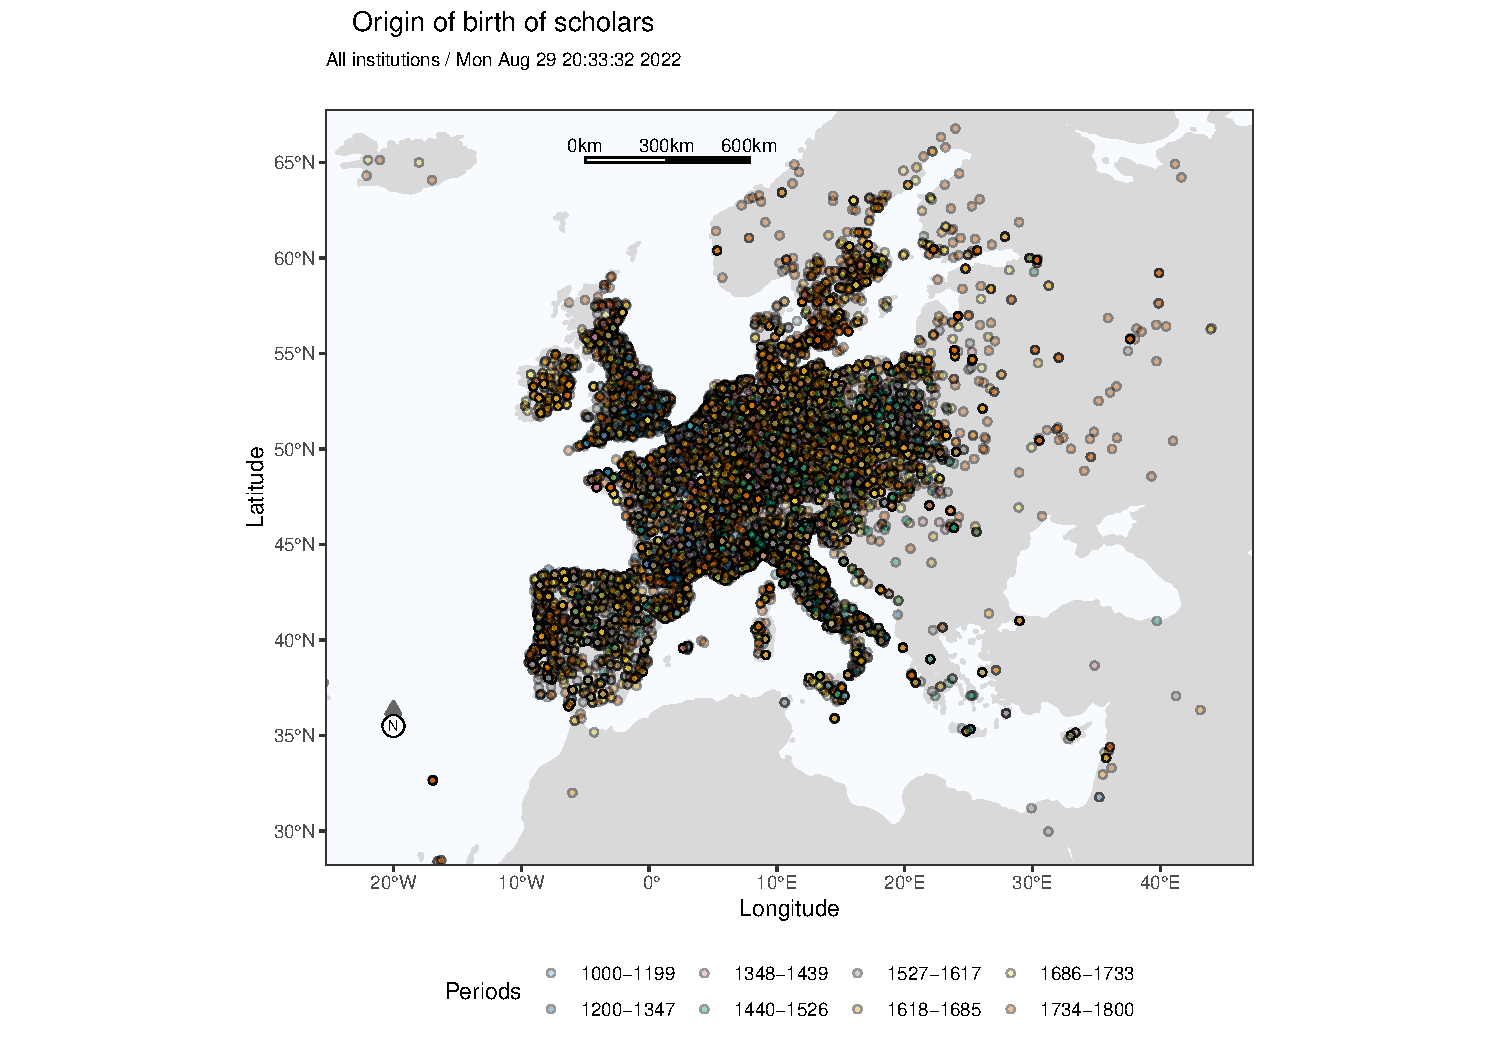
\includegraphics[width=0.9\textwidth,trim={1.5cm 0cm 2cm 1.5cm},clip]{ALL-basin(births).pdf}
\end{center}
\caption{Coverage of the European database: places of birth of scholars}\label{fig:cov}
\end{figure}


We harvested data  manually from secondary sources on the history of universities \& academies. We used a total of 522 different sources.

Some summary statistics and maps for the whole dataset are provided in \citeN{RETE}. Statistics per institution are provided in the collection \textit{Repertorium Eruditorum Totius Europae}.





\clearpage
\subsection{Sources for Thomas Dempster}\label{appendix:dempster}


\begin{figure}[!hb]
\begin{center}
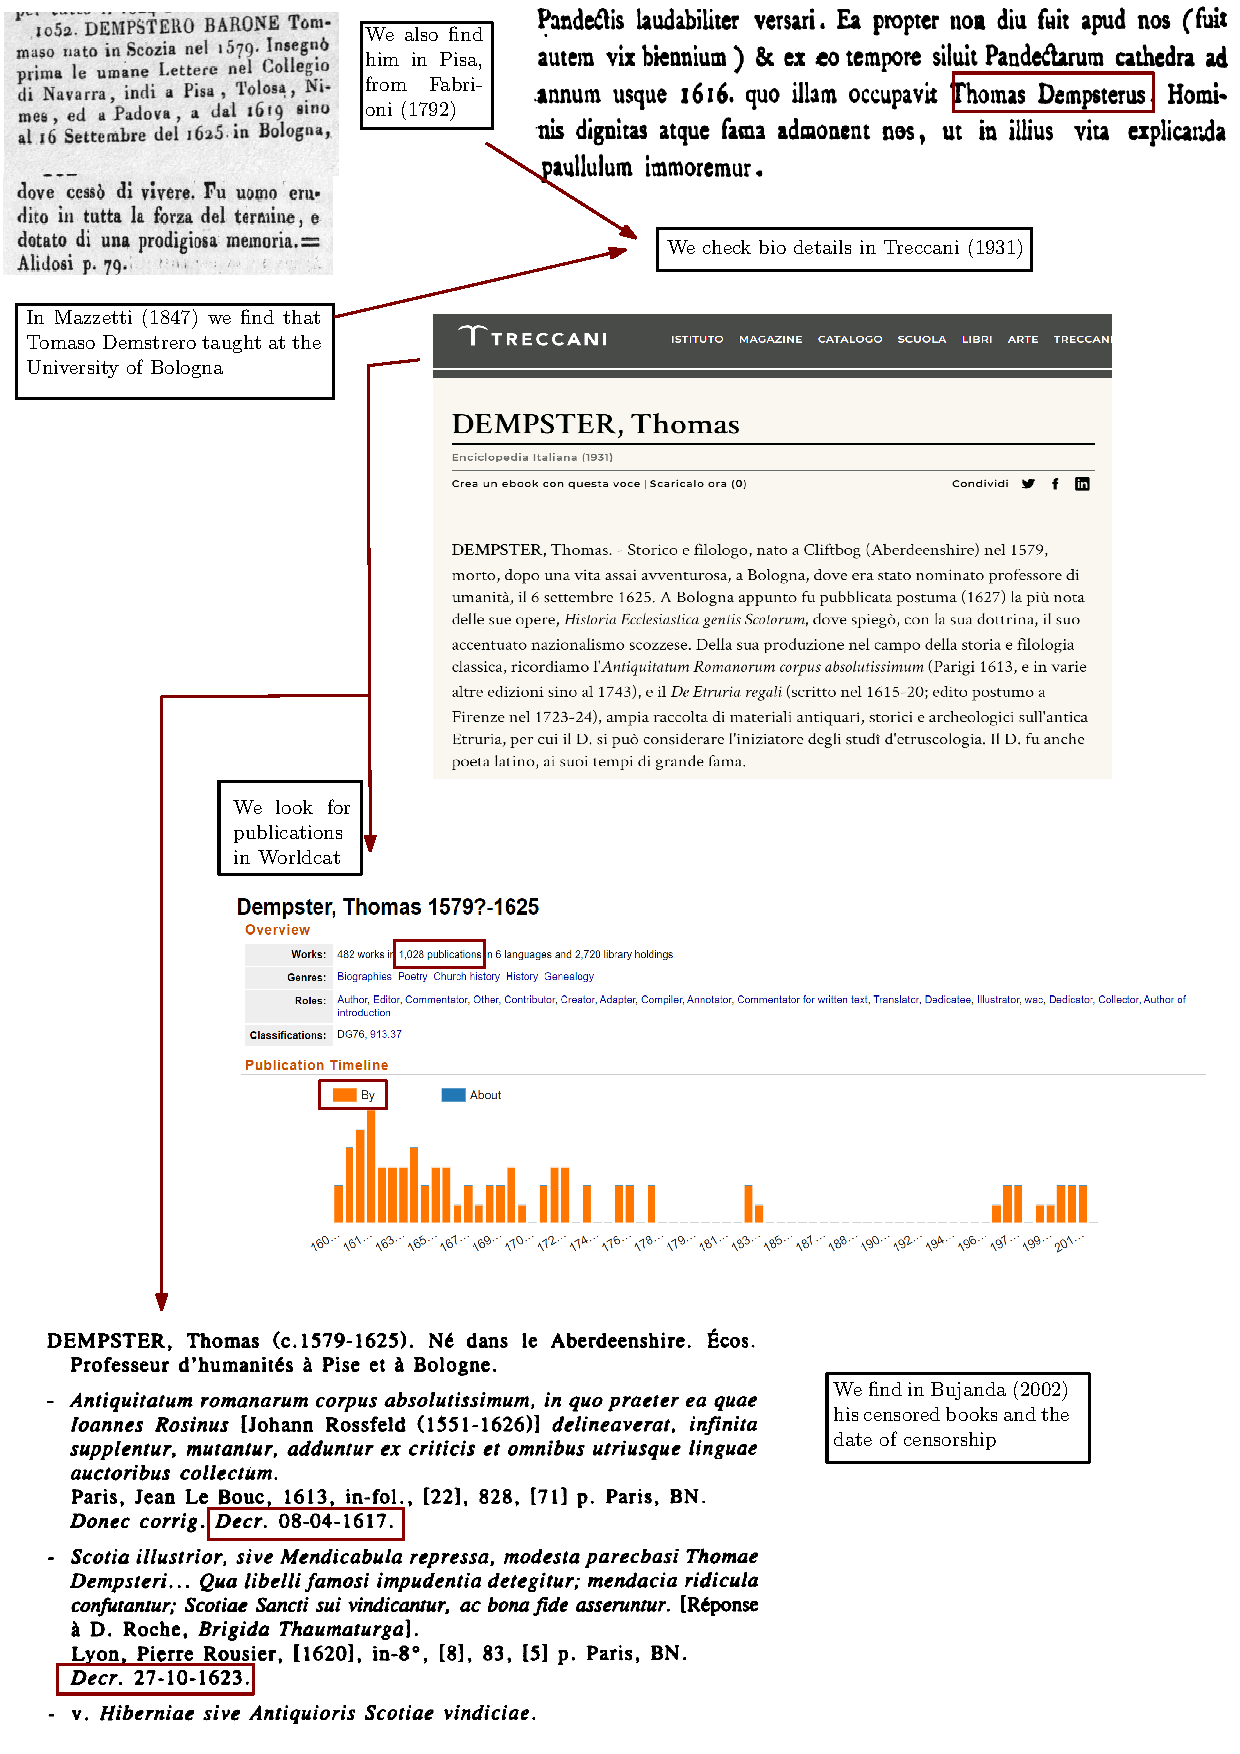
\includegraphics[width=.8\textwidth]{dempster0.pdf}
\end{center}
\caption{Data collection: example of Thomas Dempster}\label{fig:dempster}
\end{figure}


\clearpage
\subsection{How much of the Italian academic population is covered?}\label{appendix:data2}

An important question is how much of the Italian University/Academy population is covered. 

A) We believe we have a comprehensive coverage for the following universities. For each university we indicate the sources we used.


University of Bologna (1088): \citeN{mazzetti1847repertorio}. Uncertain foundation date. More details in \citeN{de2021scholarsB}.

University of Padua (1222):  \citeN{pesenti1984professori}, \citeN{casellato2002professori}, \citeN{facciolati1757fasti}, \citeN{del2015clariores}. More details in \citeN{PD2021scholars}.

University of Pisa (1343): \citeN{fabroni1795historiae}.

University of Pavia (1361):  \citeN{raggi1879memorie}, \citeN{de1961discipline}.

University of Macerata (1540): \citeN{serangeli2010docenti}. More details in \citeN{de2021scholars-mac}.

University of Roma `Gregoriana' (1556): \citeN{villoslada1954storia}.  More details in \citeN{de2021scholarsG}.


Thanks to very detailed secondary sources, we almost have all professors having taught there.

B) We have a broad coverage for the following universities.


University of Modena (1175): \citeN{mor1975storia}. For \citeN{frijhoff1996}, started as a Studium in 1682 only.

University of Naples (1224):  \citeN{paolino1754istoria}.

University of Salerno (1231):  \citeN{de1857storia}, \citeN{sinno1921diplomi}. School of medicine active before official foundation date. Unequal coverage over time, continuation of university unclear for some periods.

University of Roma 'Sapienzia' (1303): \citeN{renazzi1803storia}.

University of Perugia (1308): \citeN{Siena-www}, \citeN{zucchini2008universita},  \citeN{Onomasticon}. Comprehensive coverage of the medieval period. Broad coverage of the early modern period.

Studium in Florence (1321): \citeN{prezziner1810storia}, \citeN{cerracchini1738fasti}. No university status, but important and well documented.

University of Torino (1404): \citeN{vallauri1875storia}. More details in \citeN{zanardello2022scholars}.

University of Catania (1444): \citeN{Sabbadini-1898}, \citeN{Amari-1867}.


University of Messina (1548): \citeN{CCCL}.

University of Mondovi (1560): \citeN{vallauri1875storia}, \citeN{grassi1973dell}.


University of Palermo (1578):  \citeN{cancila2006storia},  \citeN{sommervogel1890sj}.


University of Cagliari (1606): \citeN{pillosu2017libro}, \citeN{tola1837dizionario}.


University of Sassari (1617): \citeN{mattone2010storia}.


University of Mantua (1625): \citeN{grendler2009university}, \citeN{sommervogel1890sj}.


Thanks to detailed secondary sources, we  have a large number of the professors that have taught there, and we probably have all those who published something, which is the relevant dimension for this paper.

C) For the following list, we have only a partial coverage. Many of those universities are quite small, or specialized, or detached from bigger universities (Milano \& Venice).
Ualtamura-1748,
Uancona-1562,
Ucamerino-1727,
Uferrara-1391,
Ugenoa-1773,
Ulucca-1369,
Umilano-1556,
Usiena-1246,
Uurbino-1671,
Uvenice-1470,
Uvicenza-1204.

D) For academies, assessing our coverage is more complicated, as the number of academies is potentially very large. Each city had one or more small academies, sometimes very temporarily, gathering the curious minds of the moment. As we explained in the text, our more important source comes from the data compiled by the British library based on all the books in their possession related in one way or in another to an Italian academy. To this list, we added important academies for which there is complete coverage based on a biographical dictionary of their members: the Bologna Institute, the Crusca, the Ricovrati, and the Gelati.

Accademia Platonica di Firenze (1462): \citeN{prezziner1810storia}.

Accademia Fiorentina (1540): \citeN{boutier-xls}.

Accademia della Crusca (1583): \citeN{parodi83}.

Accademia dei Gelati (1588):  \citeN{DIA}, \citeN{zanimemorie}. More details in \citeN{rolla2021scholars}.

Accademia dei Ricovrati (1599): \citeN{DIA}, \citeN{maggiolo1983soci}. More details in \citeN{blasutto2021scholars}.

Accademia degli Umoristi (1600): \citeN{DIA}.

Accademia Degli Oziosi (1611): \citeN{DIA}.

Accademia degli Incogniti (1626): \citeN{DIA}.

Scientiarum et artium institutum bonoiense atque academia (1714): \citeN{ercolani1881accademia}.  More details in \citeN{rolla2022scholars}.

and the other smaller academies included in \citeN{DIA}.



\subsection{How representative are university professors and academicians?}\label{appendix:data1}

The paper is based on publications by university professors and members of academies. One may wonder
how well those publications represent the total production of knowledge in early modern times.
To answer that question, one needs to define a new universe of persons from which we can extract the sample of university professors and compute their share.
Looking at scientific domains, let us consider the scientists who have given their name to a crater on the moon. Those names were given by the Commission on
Lunar Nomenclature of the International Astronomical Union from 1935 onward \cite{richardson1945s}.
Among these persons there are 54 Italians born before 1770. Figure~\ref{fig:moon} represents their occupation breakdown.
A large majority of them were either a university professor, a member of an academy, or both. This supports the idea that our sample of scholars is a good representation of people working in sciences.


\begin{figure}[hb]
\begin{center}
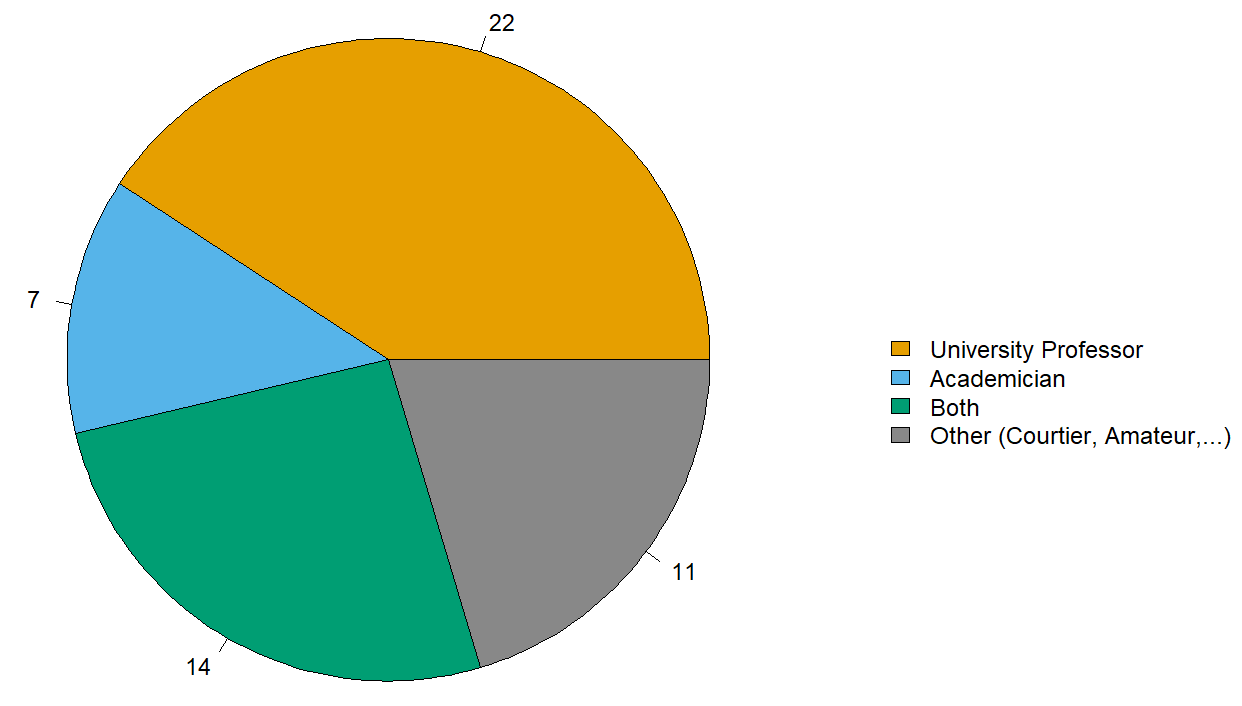
\includegraphics[width=9cm]{Erudites-Italian.png}
\end{center}
\caption{Occupations of Italians having given their name to a crater on the moon} \label{fig:moon}
\end{figure}

\clearpage
\subsection{Disaggregation of publications by institutions}\label{app:pub-by-instit}



%UPDATED 29 AUG 2022=========================================================================================================================
\begin{table}[hb]
	% Table generated by Excel2LaTeX from sheet 'Sheet1'
\centering
		\begin{tabular}{@{ \extracolsep{3pt}}lcccccccccc}
\toprule
			& \multicolumn{5}{c}{Total number of }  & \multicolumn{5}{c}{Median number of }\\
			& \multicolumn{5}{c}{published scholars}  & \multicolumn{5}{c}{ publications per person}\\
			Period   & 1 &2 & 3 & 4 & 5  & 1 &2 & 3 & 4 & 5\\
\midrule
Ubologna-1088 & 56       & 87       & 80       & 57       & 69       & 100      & 117      & 68       & 41       & 14 \\
Unapoli-1224 & 10       & 21       & 26       & 20       & 19       & 150      & 173      & 28       & 43       & 68 \\
Upadua-1222 & 76       & 131      & 132      & 76       & 81       & 83       & 82       & 79       & 55       & 23 \\
Upavia-1361 & 38       & 72       & 51       & 16       & 8        & 75       & 96       & 52       & 32       & 16 \\
Uroma-1303 & 43       & 61       & 61       & 45       & 41       & 462      & 167      & 177      & 72       & 65 \\
Upisa-1343 & 12       & 38       & 69       & 58       & 37       & 79       & 84       & 54       & 53       & 19 \\
UromaGregoriana-1556 & 0        & 0        & 65       & 53       & 51       & 0        & 0        & 189      & 84       & 25 \\
StudFlorence-1321 & 41       & 21       & 13       & 14       & 33       & 170      & 200      & 160      & 337      & 25 \\
Utorino-1404 & 14       & 15       & 30       & 3        & 38       & 53       & 107      & 119      & 12       & 17 \\
AcadRicovrati-1599 & 0        & 1        & 71       & 115      & 192      & 0        & 4        & 58       & 72       & 49 \\
AcadCrusca-1583 & 0        & 2        & 38       & 107      & 120      & 0        & 594      & 30       & 45       & 85 \\
AcadBologna-1714 & 0        & 0        & 0        & 0        & 221      & 0        & 0        & 0        & 0        & 76 \\
AcadUmoristi-1600 & 0        & 0        & 30       & 96       & 5        & 0        & 0        & 106      & 52       & 201 \\
AcadGelati-1588 & 0        & 0        & 21       & 68       & 20       & 0        & 0        & 32       & 67       & 45 \\
AcadIncogniti-1626 & 0        & 0        & 10       & 98       & 0        & 0        & 0        & 225      & 59       & 0 \\
\bottomrule
			\multicolumn{11}{l}{\footnotesize Note: periods: 1:1400-69, 2:1470-1539, 3:1540-1609, 4:1610-79, 5:1680-1749}
	\end{tabular}
	\caption{Total number of scholars \& publications by period and by Italian institution}\label{tab:publiIT}
\end{table}


\clearpage

\subsection{The decline of Italy: robustness to measurement} \label{app:robustdecline}

The first line of Table~\ref{tab:robustdecline} compares the median number of \textit{publications by}  scholars in Italy and Europe less Italy. Italy is very dominant in the first two periods, before being caught up and overtaken by the rest of Europe. The absolute decline in publications in Italy during periods 3 to 5 is impressive.

An alternative measure could simply be the \textit{number of published scholars per million inhabitants}. With this measure, the initial lead of  Italy is even more impressive. Still, Italy ends up being overtaken by period 5.

The next two  measures are computed from Worldcat. They deliver the same message as the number of \textit{publications by}. The \textit{number of works} aggregates \textit{publications by} and \textit{publications about} each scholar, but does not count the multiple editions of each work. The number of \textit{library holdings} today can be seen as a measure encompassing both output and recognition of its quality.

Finally, we computed the median \textit{number of characters of the Wikipedia pages} of the published scholars. We consider the longest Wikipedia page among European languages. Some scholars do not have a Wikipedia page, and hence the length for them is zero. There is a negative trend in Europe in the length of Wikipedia pages. For Italy, the median length goes to zero after two periods, reflecting that more than half the published Italian scholars are absent from Wikipedia (nobody wrote a page about them).


%UPDATED 29 AUG 2022=========================================================================================================================
\begin{table}[hb]
\centering
\begin{tabular}{rlrrrrr}
\toprule
          &       & \multicolumn{1}{l}{1400-69} & \multicolumn{1}{l}{1470-1539} & \multicolumn{1}{l}{1540-1609} & \multicolumn{1}{l}{1610-79} & \multicolumn{1}{l}{1680-1749} \\
          \midrule
 \multicolumn{7}{l}{Median number of publications by}\\
  & Rest of Europe & 12       & 47       & 64       & 69       & 61 \\
        & Italy    & 72       & 95       & 73       & 40       & 28 \\
\multicolumn{7}{l}{Total number of publishing scholars per million inhab.}\\
 & Rest of Europe &4.6      & 17.5     & 35.6     & 48.5     & 68.8 \\
         & Italy  &27.5     & 43.5     & 61.6     & 64.9     & 55.2 \\
\multicolumn{7}{l}{Median number of works}   \\
 & Rest of Europe & 11       & 29       & 40       & 42       & 35 \\
       & Italy    & 46       & 62       & 46       & 24       & 19 \\
\multicolumn{7}{l}{Median number of library holdings}\\
 & Rest of Europe & 48       & 119      & 144      & 151      & 154 \\
       & Italy    & 229      & 204      & 184      & 102      & 74 \\
\multicolumn{7}{l}{Median length of Wikipedia page}\\
 & Rest of Europe & 1395     & 1462     & 1087     & 985      & 953 \\
       & Italy    & 1128     & 839      & 0        & 0        & 0 \\
         \bottomrule
\end{tabular}%
\caption{The decline of Italy: robustness to measurement}\label{tab:robustdecline}
\end{table}


\subsection{Correlation between different measures of notoriety} \label{app:cor}

In this section, we use the Italian sample to compute the correlations between the various notoriety measures used in the previous section: number of publications by (Worldcat), i.e. the measure used in the main text; the number of works (Worldcat); the total number of library holdings (Worldcat); the length of the longest Wikipedia page.

We also include three additional measures not used above (because their median is constant at zero or one). The additional measures are: the number of Wikipedia pages in different languages; the number of languages involved in the publications (Worldcat), and the number of publications about (Worldcat).
Table~\ref{tab:cor} presents the linear correlations (Pearson), while table~\ref{tab:cor2} shows the rank correlations (Spearman).


\begin{table}[!htbp] \centering
\begin{tabular}{lccccccc}
\toprule
 & publi\_by & nworks & nlib & LengthWiki & NWikiLang & nlang & publi\_about \\
\midrule
publi\_by & $1$ & $0.979$ & $0.837$ & $0.394$ & $0.532$ & $0.563$ & $0.677$ \\
nworks & $0.979$ & $1$ & $0.883$ & $0.423$ & $0.588$ & $0.579$ & $0.757$ \\
nlib & $0.837$ & $0.883$ & $1$ & $0.385$ & $0.578$ & $0.525$ & $0.952$ \\
LengthWiki & $0.394$ & $0.423$ & $0.385$ & $1$ & $0.614$ & $0.443$ & $0.383$ \\
NWikiLang & $0.532$ & $0.588$ & $0.578$ & $0.614$ & $1$ & $0.624$ & $0.583$ \\
nlang & $0.563$ & $0.579$ & $0.525$ & $0.443$ & $0.624$ & $1$ & $0.482$ \\
publi\_about & $0.677$ & $0.757$ & $0.952$ & $0.383$ & $0.583$ & $0.482$ & $1$ \\
\bottomrule
\end{tabular}
  \caption{Correlations between measures of notoriety (Pearson)}
  \label{tab:cor}
\end{table}

\begin{table}[!htbp] \centering
\begin{tabular}{lccccccc}
\toprule
 & publi\_by & nworks & nlib & LengthWiki & NWikiLang & nlang & publi\_about \\
\midrule
publi\_by & $1$ & $0.984$ & $0.965$ & $0.631$ & $0.611$ & $0.795$ & $0.686$ \\
nworks & $0.984$ & $1$ & $0.954$ & $0.642$ & $0.621$ & $0.794$ & $0.703$ \\
nlib & $0.965$ & $0.954$ & $1$ & $0.675$ & $0.658$ & $0.816$ & $0.755$ \\
LengthWiki & $0.631$ & $0.642$ & $0.675$ & $1$ & $0.883$ & $0.620$ & $0.707$ \\
NWikiLang & $0.611$ & $0.621$ & $0.658$ & $0.883$ & $1$ & $0.610$ & $0.711$ \\
nlang & $0.795$ & $0.794$ & $0.816$ & $0.620$ & $0.610$ & $1$ & $0.681$ \\
publi\_about & $0.686$ & $0.703$ & $0.755$ & $0.707$ & $0.711$ & $0.681$ & $1$ \\
\bottomrule
\end{tabular}
  \caption{Rank correlations between measures of notoriety (Spearman)}
  \label{tab:cor2}
\end{table}


All the notoriety measures are highly correlated with each other, in particular when we use the rank correlation. In the main analysis, we opted for the variable ``publi by'' because it is the one which is the closest to our theoretical concept of books by an author. If we use other measures, the computed  quantiles would be similar.


\clearpage
\subsection{How is the distribution of the scholars' fields changing over time?}\label{appendix:data3}

Europe overtook Italy in terms of scholars' quality. In principle, this could be driven by the fact that a field with low average publications became relatively more common in Italy than in Europe. To answer this question, in Table \ref{tab:publi_fields} we show the dynamics of scholars' quality in Italy and Europe by field.\footnote{In case the scholar is associated with more than one field, we expand the observation according to the number of her/his fields. Details about each discipline can be found below Table \ref{tab:publi_fields}.} We observe that in each field the quality of scholars is initially lower in Europe than in Italy and that at the time censorship was introduced Italy loses (or starts losing) its advantage. Figure \ref{fig:censdis} shows that censorship affects all fields.

%UPDATED 29 AUG 2022=========================================================================================================================
\begin{table}[htb]
	\centering
	{\begin{tabularx}{\textwidth}{l *{10}{Y}}
\toprule
			&\multicolumn{5}{c}{Distribution (\%) of the scholars' fields}  & \multicolumn{5}{c}{Median publications per person}\\
			&\multicolumn{5}{c}{for each period}  & \multicolumn{5}{c}{}\\		
			Period   & 1 &2 & 3 & 4 & 5  & 1 &2 & 3 & 4 & 5\\
\midrule
			& \multicolumn{10}{c}{}\\
			& \multicolumn{10}{c}{Italy}\\
			& \multicolumn{10}{c}{}\\
   Theology & 6 & 6 & 12 & 12 & 12 & 49 & 88 & 73 & 56 & 16 \\
 Law & 39 & 27 & 20 & 13 & 14 & 68 & 81 & 22 & 6 & 15 \\
 Humanities & 35 & 41 & 45 & 49 & 37 & 132 & 131 & 97 & 49 & 39 \\
 Medicine & 13 & 16 & 13 & 13 & 15 & 58 & 66 & 73 & 65 & 24 \\
 Sciences & 7 & 9 & 9 & 12 & 20 & 31 & 63 & 165 & 70 & 44 \\
 Others & $<$1 & 1 & $<$1 & 1 & 2 &  & 747 & 52 & 16 & 13 \\
			& \multicolumn{10}{c}{}\\
			& \multicolumn{10}{c}{Europe (excluding Italy)}\\
			& \multicolumn{10}{c}{}\\
 Theology & 32 & 22 & 26 & 27 & 19 & 11 & 75 & 98 & 85 & 59 \\
Law & 24 & 18 & 18 & 14 & 12 & 6 & 23 & 46 & 59 & 72 \\
Humanities & 35 & 44 & 36 & 35 & 35 & 14 & 46 & 63 & 69 & 65 \\
Medicine & 5 & 10 & 12 & 13 & 17 & 29 & 52 & 71 & 52 & 59 \\
Sciences & 4 & 6 & 7 & 11 & 14 & 19 & 120 & 90 & 86 & 76 \\
Others & $<$1 & 1 & $<$1 & 1 & 3 &  & 12 & 378 & 125 & 74 \\
\bottomrule
			\multicolumn{11}{l}{\footnotesize Note: periods: 1:1400-69, 2:1470-1539, 3:1540-1609, 4:1610-79, 5:1680-1749.}\\
			\multicolumn{11}{l}{\footnotesize{Theology}:	Theology, scriptures}\\
			\multicolumn{11}{l}{\footnotesize{Law}:	Canon law, Roman law, French law}\\
			\multicolumn{11}{l}{\footnotesize{Humanities}:	History, Literature, Philosophy, Ethics, Rhetoric, Greek, Poetry}\\
			\multicolumn{11}{l}{\footnotesize{Medicine}:	Medicine, Anatomy, Surgery, Veterinary, Pharmacy, Botany}\\
			\multicolumn{11}{l}{\footnotesize{Sciences}:	Mathematics, Logic, Physics, Chemistry, Biology, Astronomy,  Geography}\\
			\multicolumn{11}{l}{\footnotesize {Others}: Applied Sciences (Engineering, Architecture, Agronomy),Social Sciences}
	\end{tabularx}}
	\caption{Distribution \& publications by period and field}\label{tab:publi_fields}
\end{table}


%UPDATED 29 AUG 2022=========================================================================================================================
\begin{figure}[hb]
	\centering
	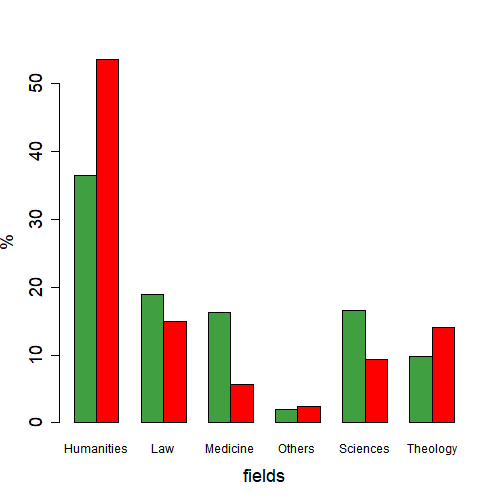
\includegraphics[width=0.7\linewidth]{cens_dis}
		\caption{Distribution of the fields of scholars. Red: censored. Green: non-censored. }
	\label{fig:censdis}
\end{figure}





\clearpage
\subsection{Famous Scholars}\label{appendix:data4}

%UPDATED 29 AUG 2022=========================================================================================================================
\begin{table}[htbp]\centering
		\begin{tabular}{lcccccccccc}%x}{\textwidth}{l *{10}{Y}}
\toprule
			& \multicolumn{5}{c}{Total number of }  & \multicolumn{5}{c}{Median number of }\\
			& \multicolumn{5}{c}{published scholars}  & \multicolumn{5}{c}{ publications per person}\\
			Period   & 1 &2 & 3 & 4 & 5  & 1 &2 & 3 & 4 & 5\\
\midrule
Europe   & 84       & 252      & 404      & 455      & 598      & 455      & 811      & 716      & 608      & 651 \\
Italy    & 41       & 77       & 137      & 115      & 122      & 680      & 828      & 637      & 453      & 594 \\
France   & 12       & 49       & 79       & 130      & 178      & 146.5    & 1113     & 988      & 520      & 670 \\
Germany \& Austria & 15       & 84       & 82       & 44       & 192      & 141      & 674.5    & 590      & 1341     & 690 \\
Great Britain \& Ireland & 3        & 21       & 50       & 119      & 242      & 15       & 607      & 493      & 808      & 564.5 \\
Denmark \& Sweden & 0        & 6        & 10       & 22       & 60       & 0        & 304      & 328      & 440      & 280 \\
Spain \& Portugal & 8        & 27       & 38       & 16       & 19       & 88.5     & 588      & 160.5    & 259      & 300 \\
Ubologna-1088 & 6        & 20       & 15       & 12       & 8        & 616.5    & 531      & 500      & 235      & 131 \\
Unapoli-1224 & 3        & 3        & 2        & 2        & 3        & 548      & 191      & 193      & 496      & 1538 \\
Upadua-1222 & 12       & 23       & 23       & 10       & 9        & 473.5    & 662      & 1105     & 388      & 563 \\
Upavia-1361 & 6        & 12       & 3        & 0        & 2        & 562.5    & 1670.5   & 656      & 0        & 980.5 \\
Uroma-1303 & 21       & 12       & 18       & 6        & 7        & 1500     & 1287.5   & 506      & 656      & 852 \\
Upisa-1343 & 0        & 7        & 9        & 9        & 3        & 0        & 758      & 493      & 438      & 245 \\
UromaGregoriana-1556 & 0        & 0        & 9        & 8        & 2        & 0        & 0        & 1582     & 1218     & 966 \\
StudFlorence-1321 & 15       & 7        & 4        & 6        & 4        & 810      & 1296     & 744.5    & 343.5    & 357.5 \\
Utorino-1404 & 1        & 1        & 4        & 0        & 4        & 553      & 935      & 1872.5   & 0        & 529 \\
AcadRicovrati-1599 & 0        & 0        & 9        & 16       & 38       & 0        & 0        & 1463     & 337      & 589.5 \\
AcadCrusca-1583 & 0        & 1        & 10       & 26       & 28       & 0        & 1184     & 644.5    & 357.5    & 685 \\
AcadBologna-1714 & 0        & 0        & 0        & 0        & 66       & 0        & 0        & 0        & 0        & 766 \\
AcadUmoristi-1600 & 0        & 0        & 6        & 24       & 0        & 0        & 0        & 2467     & 859      & 0 \\
AcadGelati-1588 & 0        & 0        & 4        & 11       & 3        & 0        & 0        & 1888     & 298      & 194 \\
AcadIncogniti-1626 & 0        & 0        & 4        & 13       & 0        & 0        & 0        & 556.5    & 540      & 0 \\
\bottomrule
			\multicolumn{11}{l}{\footnotesize Note: periods: 1:1400-69, 2:1470-1539, 3:1540-1609, 4:1610-79, 5:1680-1749}\\
			\multicolumn{11}{l}{\footnotesize Note: Famous scholars: scholars having a Wikipedia page longer than 5000 characters}
	\end{tabular}
	\caption{Total number of famous scholars \& publications by period}\label{table:europewiki}
\end{table}


\clearpage


\subsection{The gap in quality between censored and non-censored authors}\label{app:prf4}

Figure~\ref{fig:alter} below shows that before censorship was introduced in the second half of the sixteenth century, censored authors were of better quality than non-censored authors, but this gap shrank over time. Dots represent authors, which are ordered by their reference date, by log publications, and by whether or not they were censored. The two solid lines are plotted using the \textit{lowess} smoother.


%UPDATED 29 AUG 2022=========================================================================================================================
\begin{figure}[htb]
	\begin{center}
			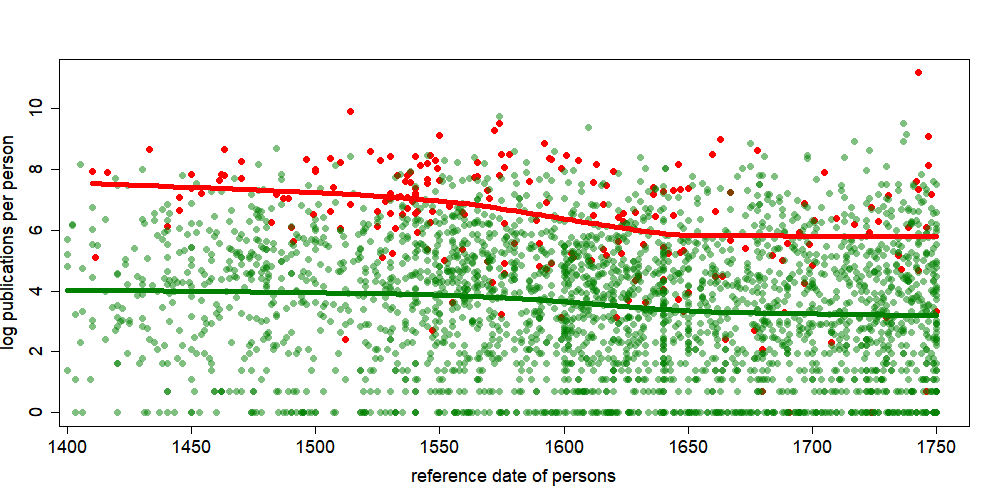
\includegraphics[width=.99\textwidth,trim=0cm 0cm 0cm 1.5cm, clip]{smoothed.png}
		\caption{Log publications of published authors by reference date. Red: censored. Green: non-censored.  Solid lines: \textit{lowess} smoother.}\label{fig:alter}
	\end{center}
\end{figure}

\clearpage

\subsection{Europe Map}\label{app:europe}


%UPDATED 29 AUG 2022=========================================================================================================================
\begin{figure}[htb]
\begin{center}
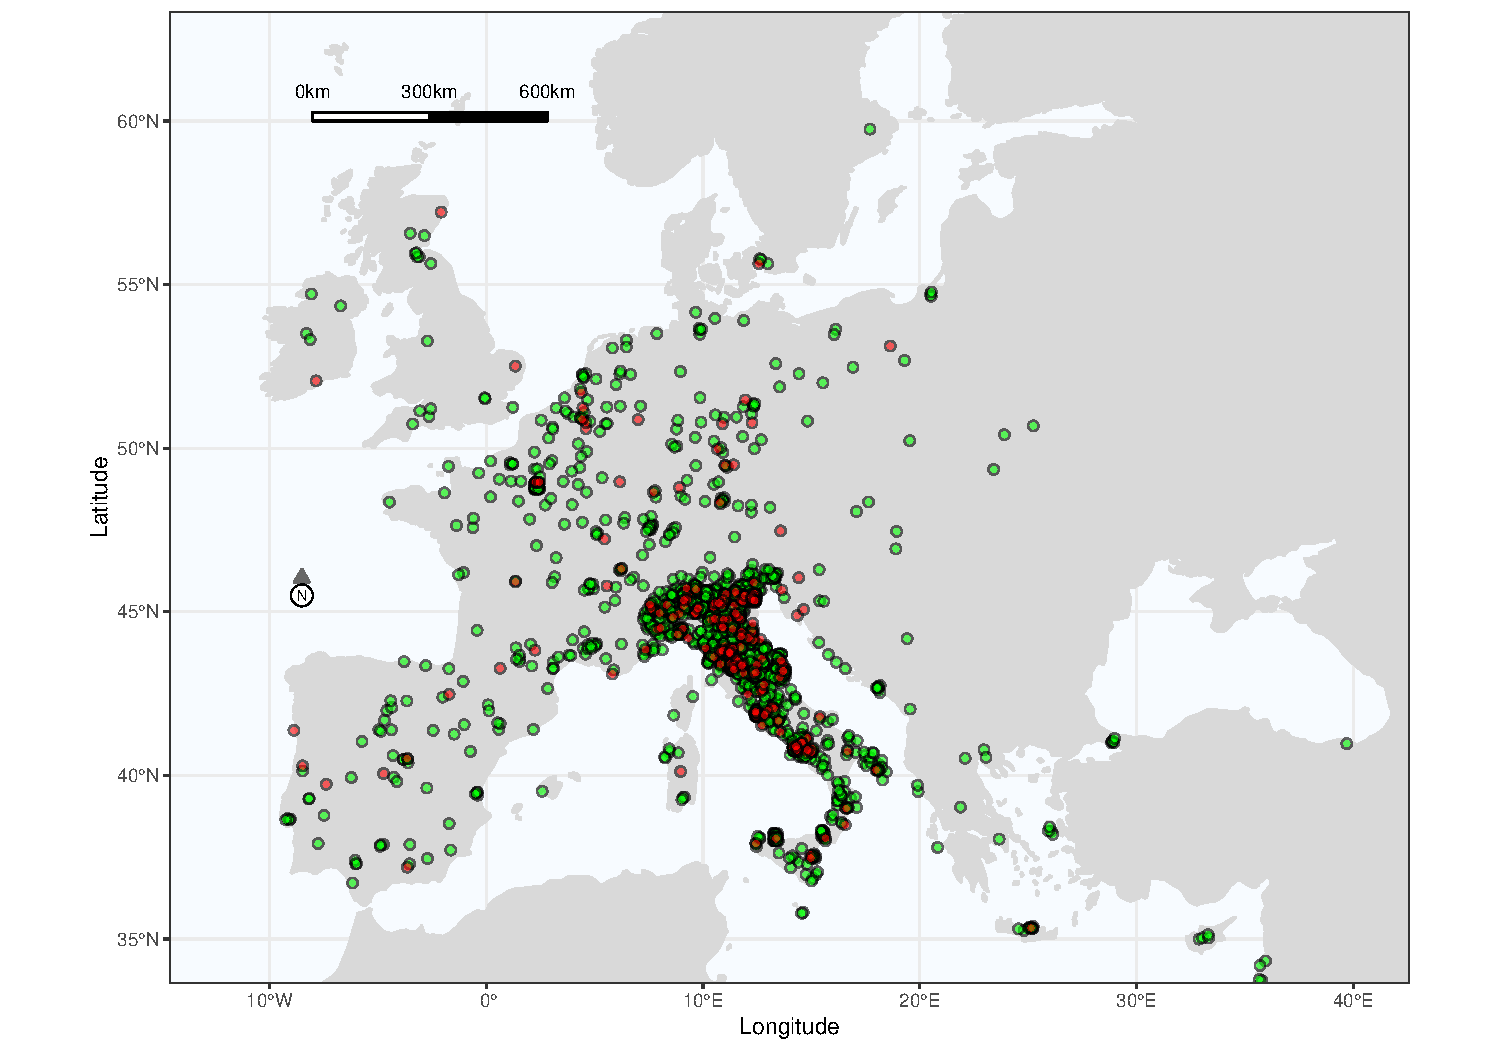
\includegraphics[width=16cm,trim=1cm 0cm 1cm 0cm,clip,angle=90,origin=c]{map-europe.pdf}
\end{center}
\caption{Place of birth of censored (red) and non censored (green) members of Italian universities \& academies  -- Europe.}\label{fig:europe}
\end{figure}

\clearpage
